\chapter{Notation}
\label{app:notation}
%\epigraph{\singlespacing \it ``It is useful to start by declaring one's notations.''}{Paul Gartner}

% \section{Indexation}
Throughout the thesis, we use the following symbols to index and label the appearing quantities:
\begin{itemize}
\item $\alpha, \beta, \gamma, \delta$: Cartesian component indices,
\item $\mu, \nu, \rho$: crystal-basis component indices,
\item $I, J$: atom number labels,
\item $i, j$: atom labels in the primitive cell,
\item ${\bf L}, {\bf K}$: lattice vectors.
\end{itemize}
We use a contra/covariant notation for vector components following Sands~\cite{Sands2002}, with an Einstein convention,
$$
{\bf x} \cdot {\bf y} = \sum_\alpha x^\alpha y_\alpha \equiv x^\alpha y_\alpha~,
$$
for sums over vector components. In particular, we have
\begin{itemize}
	\item ${\bf R}_I = (R^1_I, R^2_I, R^3_I)$: Atomic position of atom $I$ in a Cartesian components.
	\item $\set{{\bf a}_\mu}$: crystal basis with lattice vectors ${\bf a}_\mu$.
	\item $\set{{\bf a}^\mu}$: dual basis with inverse lattice vectors ${\bf a}^\mu$ fulfilling ${\bf a}^\mu \cdot {\bf a}_\nu = \delta^\mu_{~\nu}$. The cartesian components of $\set{{\bf a}^\mu}$ and $\set{{\bf a}_\mu}$ are related by
	$$ a^{\mu}_{~\alpha} = (\itp a)_{\mu \alpha} ~.$$
	\item ${\bf R}_I = R^\mu_I {\bf a}_\mu$: Atomic position of atom $I$ expressed in the crystal basis $\set{{\bf a}_\mu}$. The are $R_I^\mu$ are also called \emph{scaled} or \emph{fractional} components. They are related to the Cartesian components $R_I^\alpha$ by $R_I^\mu = {\bf a}^\mu \cdot {\bf R}_I = (\itp a)_{\mu \alpha} R_I^{\alpha}$ by the identity stated above.
	\item ${\bf L} = L^\mu {\bf a}_\mu$: A lattice vector $\bf L$ expressed in the crystal basis $\set{{\bf a}_\mu}$. 
	\item $\set{{\bf b}^\mu}$: reciprocal lattice vectors fulfilling ${\bf b}^\mu \cdot {\bf a}_\nu = 2 \pi \delta^\mu_{~\nu}$,~i.\,e.,~${\bf b}^\mu = 2\pi\,{\bf a}^\mu$ with the crystallographic convention of including the factor $2 \pi$ in the basis defintion.
	\item ${\bf q} = q_\mu {\bf b}^\mu$: phonon wave vector in the reciprocal lattice basis $\set{{\bf b}^\mu}$.
	\item ${\bf q} \cdot {\bf R}_I = 2 \pi \, q_\mu R^\mu_I$: scalar product of wave vector with atomic position.
\end{itemize}
We remind the reader that in Cartesian space, indices can be lowered and raised arbitrarily,~i.\,e.,~the components $x^\alpha$ and $x_\alpha$ are equal.

\chapter{Bloch Theorem and Brillouin Zone}
\epigraph{\singlespacing \it ``The idea of periodicity in the reciprocal space is useless but, I think, harmless.''}{Paul Gartner}
\section{Bloch theorem}
\label{sec:BlochTheorem}
The Schr\"odinger equation in 1d reads
\begin{align}
	\hat H \psi (x) = \left( - \frac{\nabla^2}{2m} + V(x) \right) \psi (x) = E \psi (x)~.
	\label{eq:app.bloch.se}
\end{align}
In a periodic potential,
\begin{align}
	V(x + a) = V(x)~,
	\label{eq:app.bloch.potential}
\end{align}
the periodicity can be expressed by stating that the translation operator $\hat T_a$ defined by its action,
\begin{align}
	\hat T_a f(x) = f(x + a)~,
	\label{eq:app.bloch.Ta}
\end{align}
commutes with the Hamiltonian,
\begin{align}
	\left[ \hat H , \hat T_a\right] = 0~.
	\label{eq:app.bloch.commute}
\end{align}
The eigenstates $\psi (x)$ of $\hat H$ are therefore also eigenstates of $\hat T_a$~\cite{Basdevant2000}. The translation operator is unitary, $\D{\hat T}_a = \hat{T}_a^{-1}$, but not hermitian. The eigenvalues $\lambda$ associated with $\hat T_a$ are thus complex numbers. By definition, one has \mbox{$\psi ( x + na ) = \lambda^n \psi(x)$}. Requiring bounded solutions, $\lim_{x \rightarrow \infty} \lvert \psi (x) \rvert < \infty$, imposes the condition $\lvert \lambda \rvert = 1$.
The function $\psi$ can therefore be written as
\begin{align}
	\psi (x) = c(x) u(x)~,
\end{align}
with a real, periodic function
\begin{align}
	u: \mathds R \rightarrow \mathds R
	\quad\text{with}\quad u(x + a) = u(x)~,
\end{align}
and a complex function of unit modulus,
\begin{align}
	c: \mathds R \rightarrow \mathds C
	\quad\text{with}\quad \left\lvert c(x) \right\rvert = 1~.
	\label{eq:app.bloch.c1}
\end{align}
We label each possible solution by the number $k$, then
\begin{align}
	c_k (x) = {\rm e}^{\im k x}
	%% don't impose uniqeness here
	%\quad\text{with}\quad k \in \left[0, \frac{2 \pi}{a} \right)
	\label{eq:app.bloch.c2}
\end{align}
% is a unique map from the domain $x \in [0, a)$ to the complex unit circle $\set{z \in \mathds C : \lvert z \rvert = 1}$. 
is a map from the domain $x \in \mathds R$ to the complex unit circle $\set{z \in \mathds C : \lvert z \rvert = 1}$. 
It then holds that $\hat T_a \psi_k (x) = {\rm e}^{\im k a} \psi(x)$,~i.\,e.,~$\psi_k$ is an eigenfunction of $\hat T_a$ with eigenvalue $\lambda = {\rm e}^{\im k a}$. We formulate the
\begin{thm}[Bloch]
	Solutions to the Schr\"odinger equation~\eqref{eq:app.bloch.se} with a periodic potential of periodicity $a$ are of the form
	\begin{align*}
		\psi_k (x) = {\rm e}^{\im k x} u_k (x)~,
	\end{align*}
	with a real, periodic function $u_k$.
%	 for each $k$ in the first Brillouin zone,
%	\begin{align*}
%		k \in \left[0, \frac{2 \pi}{a} \right)~.
%	\end{align*}
\end{thm}
The theorem is trivially extended to the 3d case by using the multiplication rule
\begin{align}
	\hat{T}_{{\bf a} + {\bf b}} f({\bf x}) = \hat{T}_{\bf a} \hat{T}_{\bf b} f({\bf x}) \equiv f({\bf x} + {\bf a} + {\bf b})~.
\end{align}
A more rigorous proof in terms of representation theory can be found,~e.\,g.,~in~\cite{Dresselhaus2007}.

\section{Brillouin Zone}
\label{sec:BrillouinZone}
We have not yet specified the range of the quantum number $k$. This can be done by requiring the complex function $c_k$ defined in Eq.\,\eqref{eq:app.bloch.c2} to map the interval $x \in [0, a)$ \emph{exactly once} to the unit circle so that $k$ is a \emph{unique} label for the eigenvalues ${\rm e}^{\im k a}$ of the translation operator $\hat T_a$.
We therefore define the
\begin{align}
	\text{Brillouin zone} = \set{k : k \in \left[ - \frac{\pi}{a}, \frac{\pi}{a}\right)}~.
\end{align}
For a wavefunction belonging to $k' = k + G$, where $G$ is an integer multiple of the the reciprocal lattice vector $b = 2\pi / a$, we would find
\begin{align}
	\hat T_a \psi_{k + G} (x) = {\rm e}^{\im k a} \psi_{k + G} (x)~.
\end{align}
They are therefore indistinguishable by the translation operator and we define $\psi_k$ and $\psi_{k+G}$ to be the same function,
\begin{align}
	\psi_k (x) = \psi_{k + G} (x)~.
\end{align}
This is sometimes termed ``periodicity of Bloch functions in reciprocal space''.



\chapter{Numerical Force Constants}
\label{app:force_constants}

\begin{marginfigure}
	\centering
	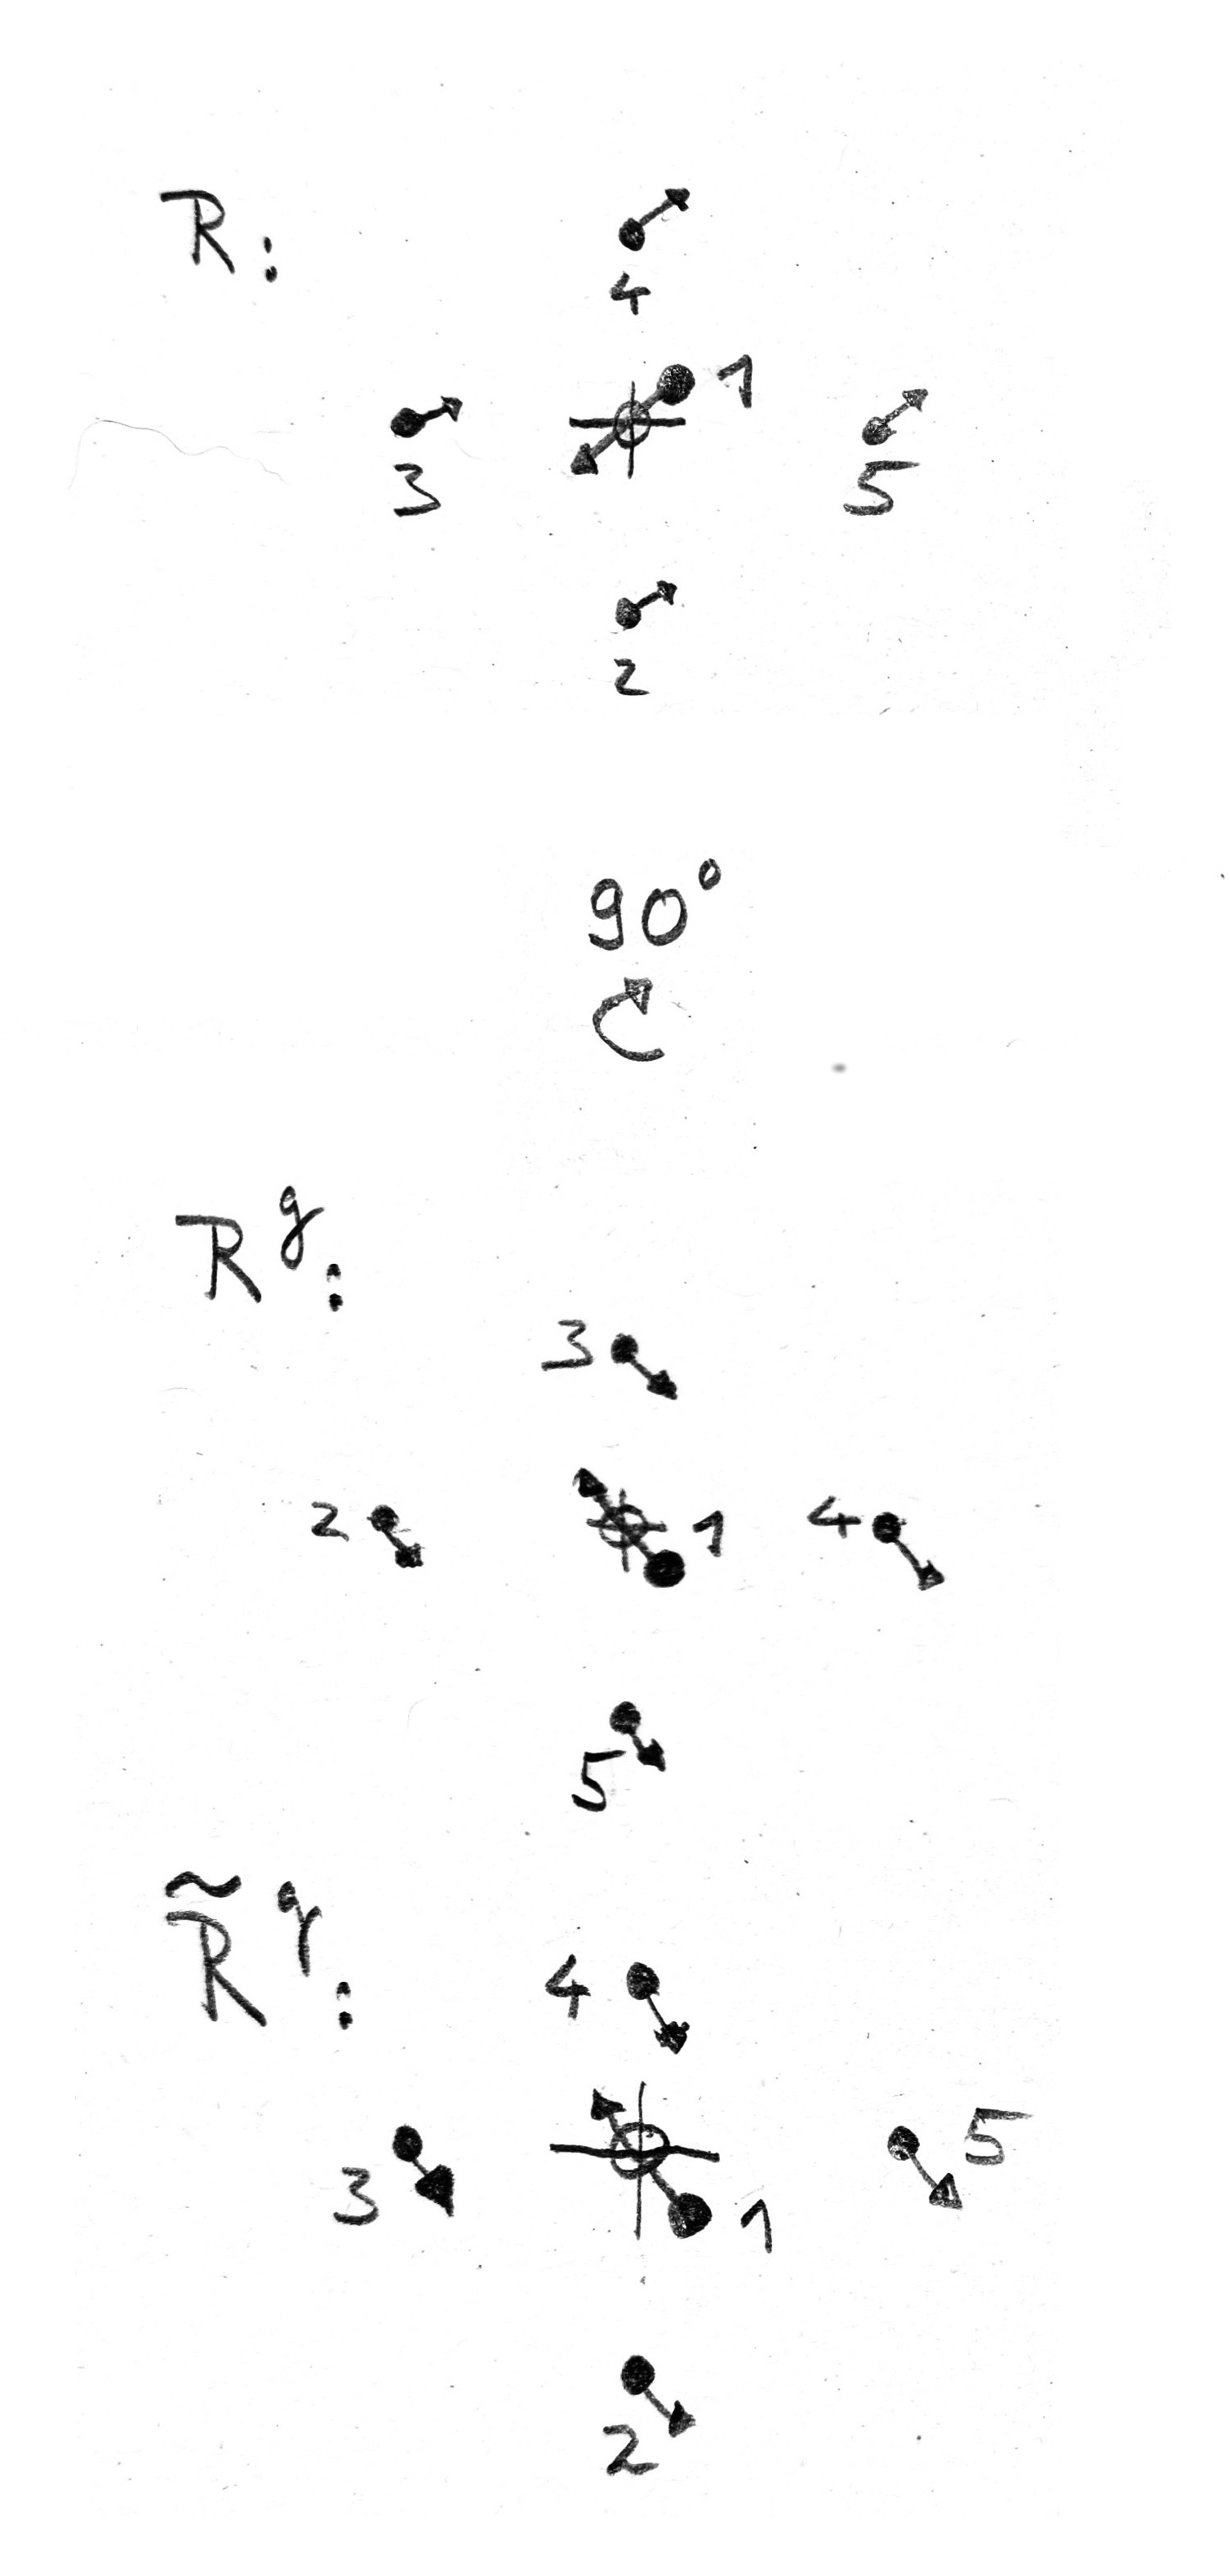
\includegraphics[width=\textwidth]{./data/sketches/symop.jpg}
	\caption{The configurations $\b R$, $\b R^g$, and $\tilde{\b R}^g$ obtained from the symmetry operation $g=\text{90 degrees rotation}$ for a two-dimensional system with five atoms. Arrows indicate the force at each atom.}
	\label{fig:symmetry.1}
\end{marginfigure}

The force constants $\Phi$ can be obtained from first-order derivatives of the potential-energy surface,~i.\,e.,~the forces, by rewriting the second derivative in terms of a finite difference expression,
\begin{align}
\Phi_{I \alpha, J \beta}
= \left.\frac{\partial^{2} \mathcal{V}(\mathbf{R})}{\partial R_{I}^{\alpha} \partial R_{J}^{\beta}}\right|_{\mathbf{R}^{0}}
= - \frac{\partial}{\partial R_I^\alpha} F_{J, \beta}
= - \lim_{\epsilon \to 0}
\frac{F_{J, \beta} (\set{\b R': R^{\prime \alpha}_I = R^{0, \alpha}_I + \epsilon )}}{\epsilon}
~.
\label{eq:FC2_finite}
\end{align}
In practice, atom $I$ is displaced by a small but finite displacement $\epsilon$ in the direction $\alpha$, and the force on all other atoms is recorded. By performing the displacement in all $3N$ degrees of freedom, the $3N \times 3N$ forces can be arranged in a matrix ${\rm F}_{[3N \times 3N]}$, and the displacements can be arranged in a matrix ${\rm U}_{[3N \times 3N]} = \epsilon \mathds 1_{[3N \times 3N]}$. The $3N \times 3N$ force-constants matrix $\Phi$ is obtained by the trivial matrix multiplication
\begin{align}
{\rm F }
&= - \Phi {\rm U} 
= - \epsilon \Phi \mathds 1
\label{eq:finite.diff.1}
\\
\implies
\Phi &= - \frac{1}{\epsilon} {\rm F} \mathds 1~.
\end{align}
%\begin{align}
%	F &= - H U \\
%	\implies
%	H &= - U^{+} F \\
%	F &= \begin{pmatrix} \b F_1, & \cdots, & \b F_{3N} \end{pmatrix}
%\end{align}
If $M > 3N$ displacements are used,~e.\,g.,~because positive and negative displacements $\pm \epsilon$ are used, the force constants can be obtained by solving an overdetermined linear equation of the kind
\begin{align}
{\rm F}_{[3N \times M]} &= - \Phi_{[3N \times 3N]} {\rm U}_{[3N \times M]} \\
\implies
\Phi &= - {\rm F} {\rm U}^{+}~,
\label{eq:phi.pseudo.1}
\end{align}
where ${\rm U}^{+}$ denotes the Moore-Penrose pseudo inverse of the displacement matrix $\rm U$~\cite{Penrose.1955,Parlinski.1997}.

\newthought{When the set of displacements and forces} $\set{ {\rm U}, {\rm F} }$ comes from thermodynamic sampling instead of finite differences, the resulting force constants $\Phi$ obtained via Eq.\,\eqref{eq:phi.pseudo.1} become temperature dependent. This is the key idea behind the \emph{temperature dependent effective potentials} (TDEP) method introduced in Ref.\,\cite{Hellman.2013}.

\section{Space group symmetry}
\label{sec:app.space-group-symmetry}
The number of required force calculations can be reduced by considering the space group symmetry of the crystal. This can be achieved in two ways: First, the symmetry can be used to identify the set of inequivalent displacements from which all other forces can be constructed by the following argument: We define the representation $\Gamma^g$ of a symmetry operation $g$ by its action on the atomic coordinates $\set{\b R_I = \b R_I^0 + \b U_I}$ as
\begin{align}
\b R_I^{g} &\equiv {\Gamma}^g (\b R_I) = { P}^g_{IJ} \b R^0_J + { M}^g \b U_I~,
\label{eq:sym.RI'}
\end{align}	
where $P^g_{IJ}$ is the permutation that relates the reference positions of atom $I$ and atom $J$, and $M^g$ is an orthogonal matrix representing the rotation (or inversion) of the respective displacement.

\newthought{As depicted in Fig.~\ref{fig:symmetry.1}}, the forces on each atom in the rotated system $\b R^g = \set{\b R^g_I}$ are obtained by co-rotating the forces in the initial configuration $\b R = \set{\b R_I}$ as
\begin{align}
\b F_I (\b R^g) &= {M}^g \b F_I (\b R)~,
\label{eq:sym.Fp}
\end{align}
i.\,e.,~the forces transform as the displacements $\b U_I$.
Let us now define a new configuration $\tilde{\b R}^g$ where just the displacements $\b U_I$ are rotated according to $g$. This can be achieved by rotating the entire system according Eq.\,\eqref{eq:sym.RI'} and applying the inverse permutation $P^{g-1}$,~i.\,e.,
\begin{align}
\tilde{\b R}_I^g 
&= P^{g-1}_{IJ} \b R_I^g 
\stackrel{\eqref{eq:sym.RI'}}{=} \b R^0_I + {\rm M}^g P^{g-1}_{IJ} \b U_J~.
\end{align}
It follows that the force on atom $I$ in the new configuration $\tilde{\b R}^g$ is related to the force in the rotated system $\b R^g$ by this inverse permutation, so that
\begin{align}
\b F_I (\tilde{\b R}^g) 
&= {P}^{g-1}_{IJ} \b F_J (\b R^g) 
= {M}^g  {P}^{g-1}_{IJ} \b F_J (\b R)~.
\label{eq:sym.Ftilde}
\end{align}
By means of this equation, the set of forces obtained for a configuration $\set{\b R_I = \b R_I^0 + \b U_I}$ can be used to generate a set of forces for each symmetrically equivalent configuration $\set{\tilde{\b R}_I^g = \b R_I^0 + {\rm M}^g P^{g-1}_{IJ} \b U_J}$, where $g$ are space group elements.

A complementary approach is to use the symmetry elements $\set{g}$ to reduce the forceconstant matrix to an irreducible basis,
\begin{align}
\Phi 
= \sum_{i=1}^{D} p_i \tilde{\Phi}_i~,
\label{eq:sym.Phi.irrep.1}
\end{align}
where the $\tilde{\Phi}_i$ are \emph{solely} determined by the space group elements $\set{g}$ and analytical properties of the forceconstants, and only the \emph{irreducible components} $p_i$ are system dependent. The pseudoinverse procedure given in Eq.\,\eqref{eq:phi.pseudo.1} then only has to be performed for the $D$ parameters $p_i$~\cite{Parlinski.1997}. This procedure can drastically reduce the number of free parameters in the forceconstant matrix. For example, in a $4\times4\times4$ bcc lattice with 128 atoms, $\Phi$ is a matrix with $(3 \cdot 128)^2 = 147456$ elements. However, there are only $D=11$ irreducible parameters $p_i$ that need to be determined~\cite{Hellman.2013}. For an exposition of the practical implementation of symmetry reduction of this kind, see for example Ref.\,\cite[p.\,25\,ff]{ErikssonThesis}.


\chapter{Geometry Optimization for Crystals}
\section{Lattice optimization at zero temperature}
\label{sec:ltrm}
The task of geometry optimization is to find a local minimum $\b R^0$ of the potential-energy surface $\mathcal{V} (\b R)$. From a mathematical point of view, $\mathcal V (\b R)$ is a function of the $3N$ coordinates $\b R$, or, when lattice degrees of freedom are included, $3N + 9$ degrees of freedom.\footnote{When rotations are rigorously excluded, the lattice only has 6~degrees of freedom.} Summarizing the positional degrees of freedom including the lattice in the generalized coordinate
\begin{align}
x 
= \left( R_{0}^x, R_{0}^y, \ldots, R_{N}^z; a^x_{~1}, a^x_{~2}, \ldots, a^z_{~3} \right) ~,
\label{eq:opt.x}
\end{align}
we seek to find
\begin{align}
x^0 = \arg \min_x \mathcal V (x)~.
\end{align}
The standard tools to solve this problem are very well covered in the standard reference~\cite{nocedal2006}. The technical pitfalls when optimizing lattices are thoroughly discussed in~\cite{Pfrommer.1997,Tadmor.1999}.
A slightly different approach as the ones discussed in the references listed above is taken in the molecular simulations code \textsc{FHI-aims}~\cite{FHI-aims}. We therefore review this approach shortly in the following.

\newthought{Many optimization algorithms} working with gradients as input are based on the Newton descent method in which the target function is locally approximated by a second-order Taylor expansion~\cite{nocedal2006}. In our case, we denote the generalized force as $f_x$ and the Hessian matrix of second derivatives as ${\rm H}_{xx'}$, where
\begin{align}
f_x 
&= - \partial_x \mathcal V (x)~,
\label{eq:opt.f} \\
{\rm H}_{xx'} 
&= \partial_x \partial_{x'} \mathcal{V} (x)~.
\label{eq:opt.H}
\end{align}
Assuming that $f_x$ and ${\rm H}_{xx'}$ are known, the neighborhood of a configuration $x$ can be written to second order in a displacement $s_x$ as\marginnote{Sum convention \mbox{$s_x f_x \equiv \sum_x s_x f_x$} is implied.}
\begin{align}
m(x + s_x) 
= \mathcal V (x) - s_x f_x + \halb \fD s_x \fD {\rm H}_{xx'} \fP s_{x'}~.
\label{eq:opt.m}
\end{align}
The minimum of this function is given by
\begin{align}
s_x = {\rm H}_{xx'}^{-1} \fD f_{x'}~,
\end{align}
which is the essence of the Newton method. One beneficial property of the Newton method is that the exact Hessian $\rm H$ is not required to be known, and one can find approximate matrices $\rm B$ that yield good results. Replacing the exact $\rm H$ by an approximate matrix $\rm B$ is known as the \emph{quasi}-Newton method.
Typically, an initial approximate Hessian $\rm B^0$ is chosen to be of simple form,~e.\,g.,~a constant times unit matrix, or based on some simpler model~\cite{Lindh.1995}. The initial guess is then updated during the optimization, for example by means of the  Broyden–Fletcher–Goldfarb–Shanno (BFGS) algorithm.\footnote{BFGS update for the estimated Hessian $B^i$ from step $i$ to $i+1$:
	\begin{align*}
	{\rm B}^{i + 1}_{xx'}
	= {\rm B}^i_{xx'} 
	& + \frac{{\rm B}^i_{x\fP{y}} s^i_{\fP{y}} s^i_{y'} {\rm B}^i_{y'x'} }{s^i_{\fP y} {\rm B}^i_{yy'} s^i_{y'}}
	- \frac{\delta f^i_{\fP x} \delta f^i_{x'}}{\delta f^i_{\fP x} s^i_{x'}}~,
	\end{align*}
	with $\delta f^i = f^{i+1} - f^i$.
}
The configuration $x$ is updated according
\begin{align}
x^{i+1} = x^i + s_x^i = ~x^i + {\rm B}^i_{xx'} f^i_{x'}.
\end{align}

\newthought{If the lattice degrees of freedom} are represented by the Cartesian components $a^\alpha_i$ of the lattice vectors, the generalized force on the lattice is given by\marginnote{Symbolically:
	$$
	f_a 
	= -\frac{\partial \mathcal V}{\partial a} 
	= -V \underset{\fD \sigma}{\underbrace{\frac{1}{V}\frac{\partial \mathcal V}{\partial \varepsilon}}} \underset{\itp a}{\underbrace{\frac{\partial \varepsilon}{\partial a}}}~.
	$$
}
\begin{align}
f_a = - V \sigma \itp{a}~,
\end{align}
where $V = \det a$ is the unit cell volume, $\sigma$ is the $3 \times 3$~stress tensor, and $a$ is the lattice matrix.\footnote{The lattice matrix is the collection of lattice vectors $\set{\b a_i}$,
	\begin{align}
	a = \begin{pmatrix} \b a_1, \b a_2, \b a_3 \end{pmatrix}~.
	\end{align}
}
For non-cubic systems, a diagonal Hessian matrix $B^0 = c \mathds 1$ will therefore produce steps proportional to the reciprocal cell $\itp{a}$ which, among other things, can break the space-group symmetry of the crystal. This behavior can be avoided by defining the initial Hessian as
\begin{align}
B^0 = c \itp{a} a^{-1}~,
\label{eq:opt.B0.new}
\end{align}
where $c$ is a numerical constant. This particular choice of $B^0$ can be viewed as making the Hessian diagonal in the native coordinate system of the lattice,~i.\,e.,~when deformations of the lattice are viewed as strain transformations in terms of the strain tensor $\varepsilon$. By the choice of the Hessian according to Eq.\,\eqref{eq:opt.B0.new}, the resulting steps $s^i_a$ will mimic such strain transformations early during the optimization:
\begin{align}
a^{i + 1} = a^i + s_a^i = (\mathds 1 + \varepsilon_s^i) a^i~.
\end{align}
Another detail that must be taken into account is that updates of the lattice necessarily have to keep the relative atomic positions expressed in the crystal basis,~i.\,e.,~their fractional coordinates, unchanged. The ideas outlined in this section have been implemented in~\textsc{FHI-aims} and the performance compared to the previous implementation is shown in Fig.\,\ref{fig:ltrm}.
\begin{marginfigure}
	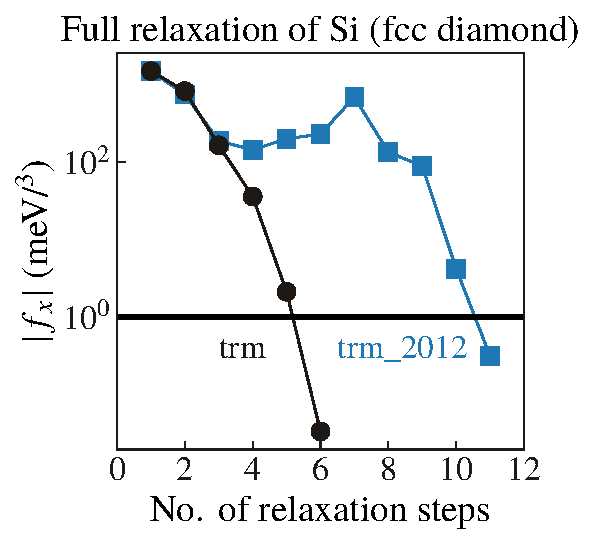
\includegraphics[width=\textwidth]{./data/plots/relaxation/ltrm.pdf}
	\caption{Residual force component as function of the relaxation steps, before (\texttt{trm\_2012}) and after (\texttt{trm}) optimizing the relaxation routine in \textsc{FHI-aims} according to the considerations presented in this chapter.}
	\label{fig:ltrm}
\end{marginfigure}
The non-systematic decrease of the residual force observed in the previous implementation (\texttt{trm\_2012}) was due to spurious distortions of the lattice and dislocations of the atomic arrangements generated by keeping their \emph{Cartesian} instead of \emph{fractional} positions unchanged during the lattice update. These artifacts are absent in the updated implementation (\texttt{trm}). The force convergence is generally faster and better behaved.


\section{Lattice optimization at finite temperature: Lattice expansion}
\label{sec:app.lattice_expansion}
At finite temperatures,\marginnote{The volume expansion is usually measured in terms of the \emph{thermal expansion coefficient} $\alpha (T)$~\cite{Kittel1969}
	\begin{align}
	\alpha (T) = \frac{1}{3 V} \frac{\partial V (T)}{\partial T}~.
	\label{eq:lattice.expansion.coefficient}
	\end{align}
}
the nuclear motion results in dynamical pressure $p(T)$ and the lattice reacts by deforming,
\begin{align}
a (T) = \bm ( \mathds 1 + \varepsilon (T) \bm ) a_0~,
\label{eq:lattice.T}
\end{align}
where $a_0$ is the 0\,K static lattice matrix, and $a (T)$ is the lattice at finite temperature given in terms of a \emph{strain transformation} $\varepsilon (T)$. 
The energy change per unit volume $\d W$ of a system subject to an infinitesimal strain deformation $\varepsilon$ is defined as
\begin{align}
\d W = \sigma_{\alpha}^{~\beta} \d \varepsilon^{\alpha}_{~\beta}~,
\label{eq:stress.strain}
\end{align}
where $\sigma$ is the \emph{stress tensor} of the system. The lattice $a(T)$ in thermal equilibrium will therefore be the lattice that minimizes the stress $\sigma$ in Eq.\,\eqref{eq:stress.strain}. Depending on the crystal symmetry~\cite{Nye1985}, the strain tensor $\varepsilon$ has up to six independent values. Equation\,\eqref{eq:stress.strain} therefore poses a six-dimensional optimization problem at a given temperature~$T$ which can be solved for example by coupling the system to a barostat and performing an $NPT$ simulation~\cite{FrenkelSmit}. In the language of the previous chapter, the lattice $a(T)$ is then given as a time or ensemble average $\braket{a}_{(p, T)}$ at thermodynamic conditions $(p, T)$. In practice however, this approach is quite inefficient and suffers from large noise, especially in the system sizes typically available to \emph{ab initio} MD simulations.

\newthought{An approximate solution} to the six-dimensional optimization problem of finding the finite temperature lattice $a (T)$ can be  found by the following rationale: We assume that the thermodynamic pressure at a given volume $V$ and temperature $T$ is given as
\begin{align}
p (V, T) \approx \frac{N k_{\rm B} T}{V} + p_{\rm pot} (V_0, T) + p_{\rm int}(V)~,
\label{eq:eos.p}
\end{align}
where $p_{\rm kin} (T) = N k_{\rm B} T / V$ is the kinetic pressure, and $p_{\rm pot} (V_0, T)$ is the potential part of the pressure in the system at reference volume $V_0$ which stems from the nuclear interaction $\mathcal V (\b R)$~\cite{Hansen1990}. The last term, $p_{\rm int} (V)$, is an internal pressure induced by the volume change. We assume that $p_{\rm int} (V)$ mainly stems from the lattice and is not temperature dependent. It can therefore be obtained from an equation of state parametrized at 0\,K, for example the \emph{Vinet equation}~\cite{Vinet.1987}:
\begin{align}
p_{\rm int} (V) 
&= \frac{3 B_0}{X^2} (1-X) {\rm e}^{\eta (1-X)} \label{eq:p.Vinet} \quad\text{with} \\ 
X &= \left[\frac{V}{V_0}\right]^{\frac{1}{3}}
\quad\text{and}\quad
\eta 
= \frac{3}{2} \left(B_0' - 1 \right)~,
\end{align}
where $V_0$ is the volume, $B_0$ is the bulk modulus, and $B_0' = \partial B_0 / \partial p$ is the isothermal pressure derivative of the bulk modulus. All these three parameters are obtained for the static lattice and we neglect their temperature dependence. Once the full parametrization of Eq.\,\eqref{eq:eos.p} is known, the temperature-dependent volume $V_{\rm min} (T)$ is found by requiring zero pressure. The resulting pressure $p_{\rm int} (V_{\rm min})$ can be used to find the static reference lattice $a(T)$ by optimizing the geometry while applying the external pressure $p_{\rm relax} = - p_{\rm int} (V_{\rm min})$ as depicted in Fig.\,\ref{fig:lattice.expansion}.
\begin{marginfigure}
	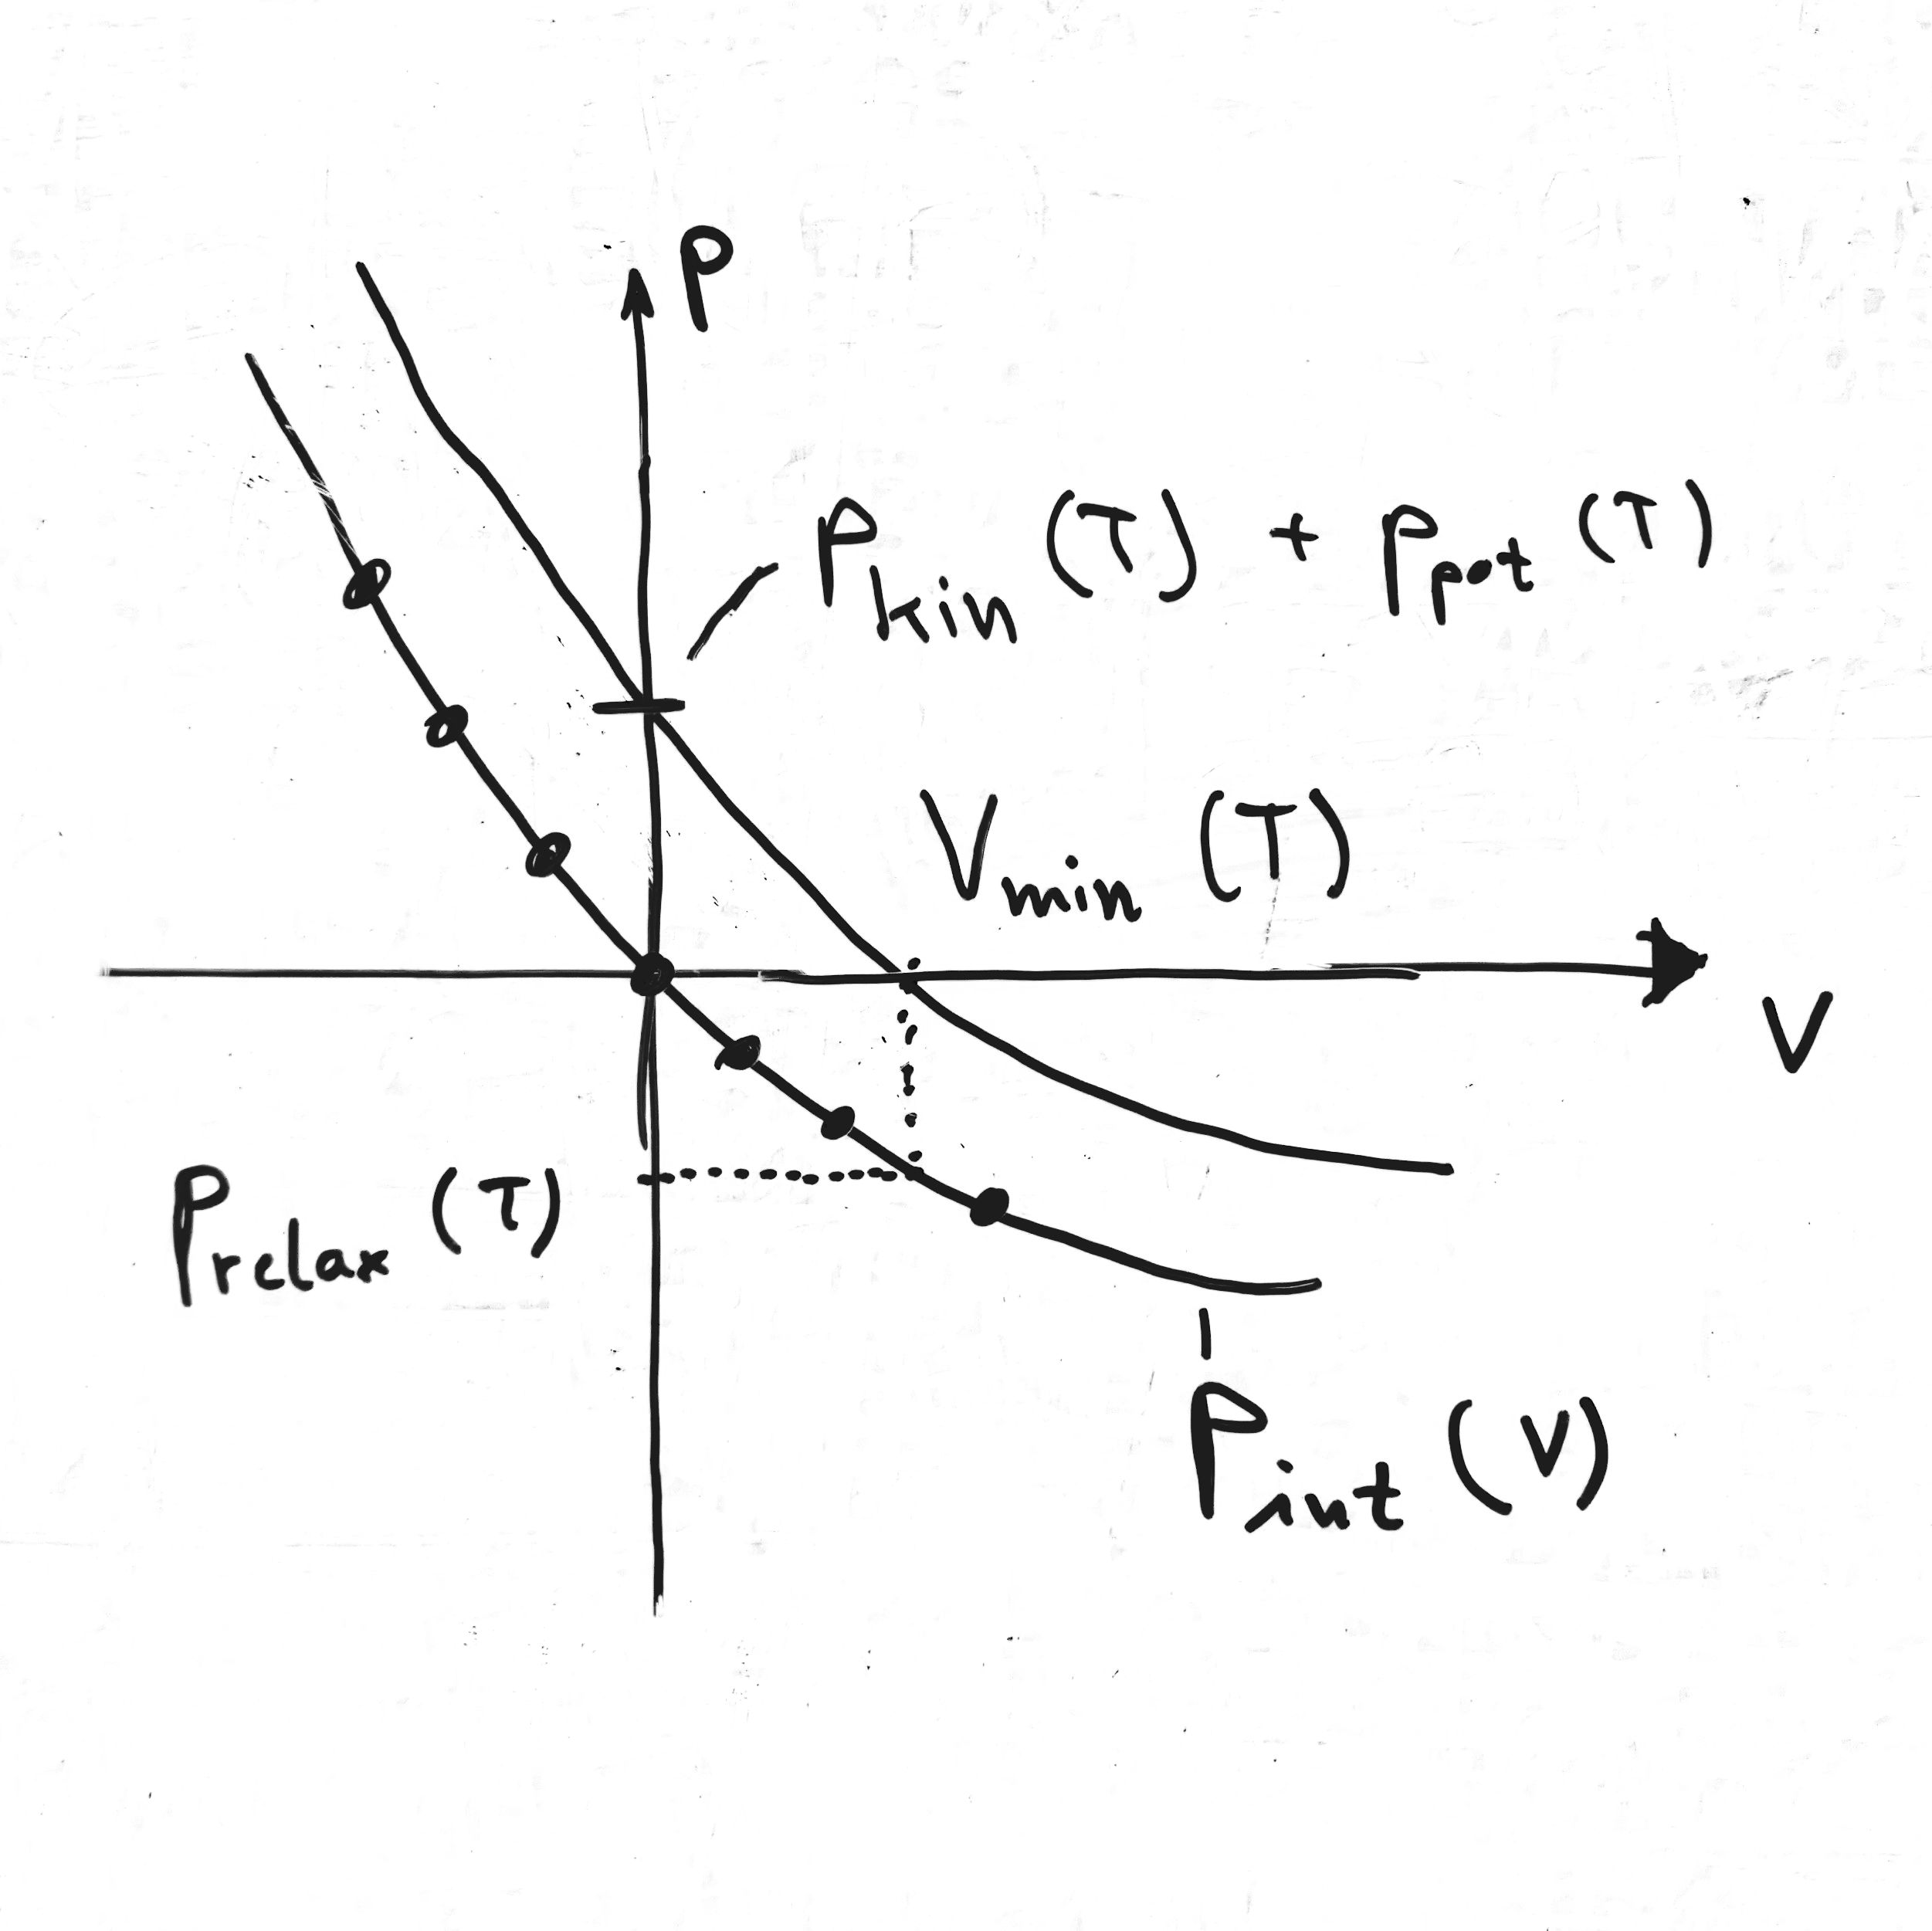
\includegraphics[width=\textwidth]{./data/sketches/lattice_expansion.jpg}
	\caption{Determination of relaxation pressure to obtain lattice at finite temperature. Dots denote volumes used to parametrize Eq.\,\eqref{eq:p.Vinet}.}
	\label{fig:lattice.expansion}
\end{marginfigure}
The lattice $a (T)$ obtained this way will then generate the static pressure contribution $p_{\rm int}$ which compensates the dynamical contributions stemming from kinetic and potential energy.

\newthought{The procedure goes as follows}:
\begin{enumerate}
	\item To parametrize $p_{\rm int} (V)$, calculate a $p(V)$ curve for different volumes\footnote{For non-cubic systems or systems with internal degrees of freedom, use a set of external pressures $p_{\rm relax}$ to obtain a set of reference structures at different volumes $V_{p_{\rm relax}}$ by geometry optimization.} and fit the Vinet equation of state given by Eq.\,\eqref{eq:p.Vinet} to obtain $(V_0, B_0, B_0')$.
	\item Perform MD simulation at $V_0$ and target temperature $T$ until pressure $p_{\rm pot} (V_0, T)$ is sufficiently  converged.
	\item Minimize Eq.\,\eqref{eq:eos.p} with respect to volume to find $V_{\rm min} = \arg \min_V p (V, T)$.
	\item Predict pressure $p_{\rm relax} = - p_{\rm int} (V_{\rm min})$ and obtain a reference structure of correct volume $V_{\rm min}$ by applying this pressure during a geometry optimization, see Fig.\,\ref{fig:lattice.expansion}. The lattice of this structure will satisfy $\det a(T) = V_{\rm min}$.
\end{enumerate}

\newthought{After the lattice $a (T)$ is obtained}, it should be verified that the pressure $p (V_{\rm min}, T)$ is indeed minimized. If a significant residual pressure $p_{\rm residual}$ persists it can be added to the pressure used for relaxation until self consistence is reached.

\chapter{Linear Response Theory}
\label{app:linear_response}

The aim of linear response theory is to compute the expected value of a phase-space observable $B$ in presence of an external perturbation driving the system out of equilibrium. The ensemble is characterized by a \emph{distribution function} $f(\Gamma, t)$, where $\Gamma = \set{\b R, \b P}$ is a shorthand for a point in phase space. The expectation value of $B$ as defined in Eq.\,\eqref{eq:phase.space.average} is given by
\begin{align}
  \braket{B (t)}
    = \int \d \Gamma ~ B (\Gamma) f(\Gamma, t)~,
  \label{eq:app.lr.B.1}
\end{align}
and we assume without loss of generality that its equilibrium value vanishes,
\begin{align}
\braket{B (t)}_{0}
= \int \d \Gamma ~ B (\Gamma) f^0(\Gamma) = 0~,
\label{eq:app.lr.B0}
\end{align}
where $f^0 (\Gamma)$ is the distribution function of the unperturbed system in thermal equilibrium. In order to calculate Eq.\,\eqref{eq:lr.B.1} in a non-equilibrium situation, we start by defining the Hamiltonian describing the dynamics of the system in the absence of external perturbations, $\mathcal H^0$, which we take to be given by the many-body Hamiltonian
\begin{align}
  \mathcal H^0 (\Gamma) 
    %= H^0(\set{\b R, \b P})
    = \sum_I \frac{\b P_I^2}{2 M_I} + \mathcal V (\b R)~.
  \label{eq:app.lr.H0}
\end{align}
The canonical distribution function for the unperturbed system reads
\begin{align}
f^0 (\Gamma) 
= \frac{1}{\mathcal{Z}^0} {\rm e}^{- \beta \mathcal H^0 (\Gamma)}~,
\label{eq:app.lr.f0}
\end{align}
where the partition function $\mathcal{Z}_0$ normalizes the phase-space integral, \mbox{$\int \d \Gamma f^0 (\Gamma) = 1$}.
In the next step, we write the full Hamiltonian as
\begin{align}
  \mathcal H (\Gamma, t)
   = \mathcal H^0 (\Gamma) + \lambda \mathcal H' (\Gamma, t)~,
  \label{eq:app.lr.H}
\end{align}
where the perturbation is given by some yet unspecified phase-space function $\mathcal H' (\Gamma, t)$ with explicit time dependence, and $\lambda = 1$ is a bookkeeping parameter that we introduce to count the order in the perturbation.

We write the distribution function in presence of the perturbation as
\begin{align}
  f (\Gamma, t) = f^0(\Gamma) + \lambda \Delta f (\Gamma, t)~,
  \label{eq:app.lr.f}
\end{align}
where $\Delta f$ is the perturbation in the distribution generated by $\mathcal  H'$. Using that $f^0$ carries no explicit time dependence, the Liouville equation for $\Delta f$ reads
\begin{align}
  \lambda \frac{\d \Delta f}{\d t}
    &= \set{\mathcal  H, f} \nonumber \\
    &= \lambda \set{\mathcal H^0, \Delta f} 
      + \lambda \set{\mathcal H', f^0}
      + \mathcal{O}(\lambda^2)~,
  \label{eq:app.lr.df.1} \\
  \implies
    \frac{\d \Delta f}{\d t}
      &\approx \set{\mathcal H^0 , \Delta f} + \set{\mathcal H' (t), f^0}
  \label{eq:app.lr.df.2}
\end{align}
where $\set{\cdot , \cdot}$ denotes the Poisson bracket
%\footnote{
%  The Poisson bracket for a system of particles with $3N$ positions $q_i \equiv R_I^\alpha$ and conjugate momenta $p_i \equiv P_I^\alpha$ reads
%  $$
%  \set{A, B} = \sum_{i}
%  \frac{\partial A}{\partial q_i} \frac{\partial B}{\partial p_i}
%  - \frac{\partial A}{\partial p_i} \frac{\partial B}{\partial q_i}~.
%  $$
%  }, 
and in Eq.\,\eqref{eq:app.lr.df.2} we only keep the terms to linear order in the perturbation.
The solution to this differential equation is found to be\footnote{The solution is given below in Sec.\,\ref{app:lr.f}.}~\cite{Kubo1957a}
\begin{align}
  \Delta f (\Gamma, t) 
    = \int_{-\infty}^t {\rm e}^{-\im \mathcal  L^0 (t - t')} \set{\mathcal  H' (\Gamma, t'), f^0 (\Gamma)}~\d t'~,
  \label{eq:app.lr.df(t)}
\end{align}
where ${\rm e}^{\im \mathcal  L^0 t}$ propagates a phase-space point $\Gamma$ by a time $t$ according to the equations of motion following from $\mathcal H^0$.
By splitting the interaction Hamiltonian $\mathcal H'(t)$ into an operator part $ A(\Gamma)$ and an explicitly time dependent force function $F(t)$,
\begin{align}
  \mathcal H' (\Gamma, t)= A (\Gamma) F(t)~,
  \label{eq:app.lr.H_AF}
\end{align}
equation~\eqref{eq:app.lr.df.2} can be simplified in the canonical ensemble by using that \mbox{$\partial f^0 / \partial \mathcal H^0 = -\beta f^0$}, which leads to\footnote{This can be seen by using the chain rule and the canonical equations of motion:	
\begin{align*}
	\set{A, f^0}
	&= \sum_i \frac{\partial A}{\partial q_i} \frac{\partial f^0}{\partial p_i}
	- \frac{\partial A}{\partial p_i} \frac{\partial f^0}{\partial q_i} \\
	&= \sum_i \frac{\partial A}{\partial q_i} \frac{\partial f^0}{\partial H^0} \frac{\partial H^0}{\partial p_i}
	- \frac{\partial A}{\partial p_i} \frac{\partial f^0}{\partial H^0} \frac{\partial H^0}{\partial q_i} \\
	&= -\beta f^0 \sum_i
	\left( \frac{\partial A}{\partial p_i} \dot{q}_i +  \frac{\partial A}{\partial q_i} \dot{p}_i \right) \\
	&= -\beta f^0 \, \frac{\d A}{\d t} \\
	&\equiv -\beta f^0 \, \dot A~.
	\end{align*}}
\begin{align}
  \set{A, f^0}
    &= -\beta \dot A f^0~,
   \label{eq:app.lr.dA_dt}
\end{align}
so that the Poisson bracket %of the perturbing Hamiltonian $\mathcal H'$ with the unperturbed distribution function $f^0$ 
appearing in Eq.\,\eqref{eq:app.lr.df(t)} becomes
\begin{align}
	\left\{\, \mathcal  H' (\Gamma, t'), f^0 (\Gamma) \,\right\}
		= - \beta \dot{A} (\Gamma) f^0 (\Gamma) F(t')~,
	\label{eq:app.lr.poisson.H'}
\end{align}
i.\,e., a product of minus the inverse temperature $\beta$ with the time derivative of the operator part $\dot A (\Gamma)$, the distribution $f^0 (\Gamma)$, and the time-dependent force function $F (t)$.

\newthought{We are now in position to formulate the expected response} of a phase space observable $B$ to linear order in a perturbation described by the Hamiltonian $\mathcal H'(\Gamma, t)$ defined in Eq.\,\eqref{eq:lr.H_AF},~i.\,e.,~
\begin{align}
\braket{B (t)}
    &= \int \d \Gamma ~  B (\Gamma) \Delta f (\Gamma, t) \\
    &= - \beta \int_{-\infty}^t 
      \int \d \Gamma ~  
       B (\Gamma) \, {\rm e}^{-\im \mathcal L^0 (t - t')} \dot{A}(\Gamma)
       f^0(\Gamma) F(t') ~ \d t' \\
    &= - \beta \int_{-\infty}^t 
      \braket{B(\Gamma_t) \dot{A} (\Gamma_{t'})}_{0} F(t') ~ \d t'~,
  \label{eq:app.lr.dB}
\end{align}
where $\braket{\cdot}_{0}$ denotes a phase-space average with respect to the unperturbed canonical distribution function $f^0 (\Gamma)$, and the notation implies that for each phase-space point $\Gamma$ in the ensemble, $B (\Gamma)$ and $\dot{A} (\Gamma)$ are evaluated at phase-space points separated in time by $t-t'$~\cite[p.\,498]{Tuckerman}.
%it was used that $a(t) = {\rm e}^{\im \mathcal L^0 t} a(0) = a(0) {\rm e}^{-\im \mathcal L^0 t}$, and  as before. 
%It is evident from this equation that the time propagation of the observables $\dot {A}$ and $B$ 
The time propagation of phase-space points is generated by $\mathcal L^0$ and therefore given by the canonical equations of motion with conserved energy as defined in Eq.\,\eqref{eq:stat.eom}. The phase-space average $\braket{\cdot}_{0}$ on the other hand corresponds to a canonical ensemble average with respect to the distribution function $f^0$ defined in Eq.\,\eqref{eq:lr.f0}.


\section{Perturbed distribution function}
\label{app:lr.f}
To solve for $\Delta f(t)$ defined in Eq.\,\eqref{eq:app.lr.df.2}, we introduce a shorthand notation such that
%
\begin{align}
  \frac{\d \Delta f}{\d t} = -\im \mathcal L \Delta f(t) - \im \Delta \mathcal L (t) f^0~,
  \label{eq:lr.df.3}
\end{align}
where the Liouville operator $\mathcal L^0$ is defined by
%
\begin{align}
	\im \mathcal  L^0 g = \set{g, \mathcal H^0}~,
	\label{eq:app.lr.L}
\end{align}
%
and similarly
\begin{align}
	\im \Delta \mathcal L (t) g = \set{g, \mathcal H'(t)}~.
	\label{eq:app.lr.L'}
\end{align}
Equation~\eqref{eq:lr.df.3} is a first order linear differential equation of the form
\begin{align}
	\frac{\d y}{\d t} + p(t) y = q(t)~,
	\label{eq:app.lr.dgl.1}
\end{align}
which is straightforward to solve by using an integrating factor as follows: We identify $y = \Delta f$, $p(t) = \im \mathcal L^0$, and $q(t) = - \im \Delta \mathcal L (t) f^0$. Following Ref.~\cite[p.\,68]{Lomen1986}, we define the integrating factor \mbox{$\rho (t) = \exp(\int \d t \, p (t)) = \exp (\im \mathcal L^0 t)$}, multiply Eq.\,\eqref{eq:app.lr.dgl.1} with $\rho (t)$, and use that \mbox{$\frac{\d}{\d t} \, \rho(t) = \rho(t) p(t)$} to obtain
$$
  \frac{\d}{\d t} (\rho (t) y) = \rho(t) q(t)~.
$$
This gets integrated to
$$
\rho(t) y = \int_{-\infty}^t \d t' \, \rho(t') q(t')
$$
under the boundary condition $y (t \to -\infty) = 0$. In total we obtain
%
\begin{align}
  y(t) 
    &= \rho^{-1} (t) \int_{-\infty}^t \d t' \, \rho(t') q(t')~, \\
  \implies
  \Delta f(t) 
    &= - {\rm e}^{- \im \mathcal L^0 t}  \int_{-\infty}^t \d t' \, {\rm e}^{\im \mathcal L^0 t'} \im \Delta \mathcal L (t') f^0~.
\end{align}

\chapter{Explicit Formulas}
\section{Harmonic approximation}
\label{app:formulas.ha}
In Sec.\,\ref{sec:dynmat.periodic}, we introduced the shorthand notation $s=(b, \b q)$, $-s=(b, -\b q)$ to write brief formulas. We give the explicit form of these formulas here.

\newthought{The normal mode coordinates} in the periodic case in terms of complex amplitudes $a^{(\dagger)}_b (\b q)$ read
\begin{subequations}
	\label{eq:u_b(q).amplitudes}
	\begin{align}
	u_b (\b q)
	&=   \frac{1}{\sqrt{2 \omega_b (\b q)}} \left[ \D a_b (- \b q) + \fD a_b (\b q)  \right] \\
	p_b (\b q)
	&= \im \sqrt{\frac{\omega_b (\b q)}{2}} \left[ \D a_b (- \b q) - \fD a_b (\b q)  \right]
	\end{align}
	\end{subequations}
	The inverse relation is given by
	\begin{subequations}
		% \label{eq:a(q)}
		\begin{align}
		a_b (\b q)
		&= \sqrt{\frac{\omega_b (\b q)}{2}} u_b (\b q) + \frac{\im}{\sqrt{2 \omega_b (\b q)}} p_b (\b q) \\
		a^\dagger_b (-  \b q)
		&= \sqrt{\frac{\omega_b (\b q)}{2}} u_b (\b q) - \frac{\im}{\sqrt{2 \omega_b (\b q)}} p_b (\b q)
		\end{align}
		\end{subequations}
		The displacements are recovered by
		\begin{align}
		\b u_{i \b L}
		&= \frac{1}{\sqrt{N_{\b q}}} \sum_{b \b q} {\rm e}^{\im  \b q \cdot \b R^0_{i \b L}} \, \b e^\ast_{b i} (\b q) \fD u_b (\b q)
		% \label{eq:u_iL}
		% \\
		% \b p_{i \b L}
		% &= \frac{1}{\sqrt{N_{\b q}}} \sum_{b \b q} {\rm e}^{\im  \b q \cdot \b R^0_{i \b L}} \, \b e^\ast_{b i} (\b q) \fD p_b (\b q)
		\end{align}
		%\end{subequations}
		and likewise for $\b p$.
		
		The Hamiltonian reads
		\begin{align}
		\mathcal H (u_b, p_b)
		&= \frac{1}{2} \sum_{b \b q} \left[ p^\ast_b (\b q) p_b (\b q) + \omega^2_b (\b q) u^\ast_b (\b q) u_b (\b q) \right] 
		\end{align}
		Equations of motion
		\begin{align}
		\ddot{u}_b (\b q)
		= \dot{p}_b (\b q)
		= - \frac{\partial \mathcal{H}}{\partial u_b^\ast (\b q)}
		\end{align}

\newpage

\section{Heat capacity}
\begin{subequations}
\begin{align}
	\beta
		& = \frac{1}{k_{\rm B} T} \\
	c_V 
		&= \frac{\partial E}{\partial T} \\
	E (T)
		&= \sum_s \hbar \omega_s n_s (T) \\
	n_s (T)
		&= \frac{1}{e^{\beta \hbar \omega_s} - 1} \\
	\frac{\partial n_s}{\partial T}
		&= \frac{\hbar \omega_s}{k_{\rm B} T^2} \, n_s (n_s + 1) \\
	\implies c_V
		&= \sum_s \underset{c_{V, s}}{\underbrace{\frac{\hbar^2 \omega_s^2}{k_{\rm B} T^2} \, n_s (n_s + 1)}}
\end{align}
\end{subequations}
Classical limit $k_{\rm B} T \gg \hbar \omega_s$
\begin{subequations}
\begin{align}
	n_s (T) 
		&\to \frac{k_{\rm B} T}{\hbar \omega_s} \gg 1 \\
	\implies E(T)
		&\to 3 N k_{\rm B} T \\
	\implies c_V 
		&\to 3 N k_{\rm B}
\end{align}
\end{subequations}


\chapter{Anharmonicity Screening}
\label{sec:app.screening}

Tables~\ref{tab:screening.sigma.1}--\ref{tab:screening.sigma.3} list results from the one-shot anharmonicity screening performed in Ref.~\cite{Knoop.2020}:

\begin{table}[h!]
%  \centering
%  \fontfamily{ppl}\selectfont  
\small
\begin{tabular}{rrllr}
\toprule
 Space group &  $N_{\rm primitive}$ & Material & Materialsproject ID &  $\sigmaAOS$ \\
\midrule
          56 &           20 &  Sb$_2$O$_3$ &    mp-2136 &       0.28 \\
          61 &           16 &         ZnSb &     mp-753 &       0.31 \\
          62 &            8 &         SnSe &     mp-691 &       0.35 \\
          62 &           24 &     BaSi$_2$ &    mp-1477 &       0.25 \\
          62 &           20 &     KCaF$_3$ &    mp-5926 &       0.37 \\
          62 &           20 &     KCdF$_3$ &    mp-9628 &       0.40 \\
         122 &            8 &    AgAlS$_2$ &    mp-5782 &       0.28 \\
         122 &            8 &   AgAlSe$_2$ &   mp-14091 &       0.27 \\
         122 &            8 &   AgAlTe$_2$ &   mp-14092 &       0.29 \\
         122 &            8 &    AgGaS$_2$ &    mp-5342 &       0.30 \\
         122 &            8 &   AgGaSe$_2$ &    mp-5518 &       0.30 \\
         122 &            8 &    AlCuS$_2$ &    mp-4979 &       0.24 \\
         122 &            8 &   AlCuSe$_2$ &    mp-8016 &       0.28 \\
         122 &            8 &   AlLiTe$_2$ &    mp-4586 &       0.26 \\
         122 &            8 &    CuInS$_2$ &   mp-22736 &       0.29 \\
         122 &            8 &   GaLiTe$_2$ &    mp-5048 &       0.27 \\
         122 &            8 &   InLiTe$_2$ &   mp-20782 &       0.26 \\
         164 &            5 &         MgSb &    mp-2646 &       0.31 \\
         166 &            4 &    Ba$_2$BrN & mp-1018098 &       0.41 \\
         166 &            4 &    Ba$_2$ClP &   mp-27869 &       0.29 \\
         166 &            4 &    CuGaO$_2$ &    mp-4280 &       0.21 \\
         166 &            4 &    CuScO$_2$ &    mp-4636 &       0.27 \\
         166 &            4 &   InLiSe$_2$ &   mp-10618 &       0.35 \\
         166 &            4 &    InNaO$_2$ &    mp-5175 &       0.21 \\
         166 &            4 &    InNaS$_2$ &   mp-20289 &       0.26 \\
         166 &            4 &   InNaSe$_2$ &   mp-22473 &       0.32 \\
         166 &            4 &     LiF$_2$H &   mp-24199 &       0.45 \\
         166 &            4 &    LiRhO$_2$ &   mp-14115 &       0.22 \\
         166 &            4 &    LiScS$_2$ & mp-1001786 &       0.28 \\
         166 &            4 &     NaF$_2$H &   mp-27837 &       0.41 \\
         166 &            4 &    Sr$_2$ClN &   mp-23033 &       0.28 \\
         166 &            4 &     Sr$_2$HN &  mp-690794 &       0.30 \\
         166 &            4 &     Sr$_2$IN &  mp-569677 &       0.28 \\
         166 &            5 & Bi$_2$Te$_3$ &   mp-34202 &       0.24 \\
\bottomrule
\end{tabular}
   \caption{Results from anharmonicity screening for space groups 56--166.}
   \label{tab:screening.sigma.1}
 \end{table}         
  
\begin{table}[t]
%  \centering
%  \fontfamily{ppl}\selectfont  
\small
\begin{tabular}{rrllr}
\toprule
 Space group &  $N_{\rm primitive}$  &     Material & Materialsproject ID &  $\sigmaAOS$ \\
\midrule         
         186 &            4 &          AgI &   mp-22894 &       0.42 \\
         186 &            4 &          CdS &     mp-672 &       0.27 \\
         186 &            4 &         CdSe &    mp-1070 &       0.26 \\
         186 &            4 &         MgTe &    mp-1039 &       0.26 \\
         186 &            4 &          ZnO &    mp-2133 &       0.22 \\
         186 &            4 &          ZnS &  mp-560588 &       0.22 \\
         186 &            4 &         ZnSe &     mp-380 &       0.22 \\
         206 &           40 &  Sc$_2$O$_3$ &     mp-216 &       0.23 \\
         216 &            2 &         AlAs &    mp-2172 &       0.17 \\
         216 &            2 &          CdS &    mp-2469 &       0.24 \\
         216 &            2 &         CdTe &     mp-406 &       0.26 \\
         216 &            2 &         CuBr &   mp-22913 &       0.52 \\
         216 &            2 &         CuCl &   mp-22914 &       0.55 \\
         216 &            2 &          CuI &   mp-22895 &       0.37 \\
         216 &            2 &         GaAs &    mp-2534 &       0.18 \\
         216 &            2 &         InAs &   mp-20305 &       0.21 \\
         216 &            2 &          ZnS &   mp-10695 &       0.23 \\
         216 &            2 &         ZnSe &    mp-1190 &       0.23 \\
         216 &            2 &         ZnTe &    mp-2176 &       0.25 \\
         216 &            3 &       LiAsMg &   mp-12558 &       0.27 \\
         216 &            3 &       LiAsZn &    mp-9124 &       0.26 \\
         216 &            3 &        LiNZn &    mp-7575 &       0.25 \\
         216 &            3 &        ZnPLi &   mp-10182 &       0.25 \\
         221 &            2 &         CsBr &   mp-22906 &       0.42 \\
         221 &            2 &         CsCl &   mp-22865 &       0.39 \\
         221 &            2 &          CsI & mp-1056920 &       0.40 \\
         221 &            5 &    BaLiF$_3$ &   mp-10250 &       0.27 \\
         221 &            5 &    CsCaF$_3$ &    mp-7104 &       0.26 \\
         221 &            5 &    CsCdF$_3$ &    mp-8399 &       0.32 \\
         221 &            5 &     KMgF$_3$ &    mp-3448 &       0.24 \\
         221 &            5 &     KZnF$_3$ &    mp-5878 &       0.32 \\
         221 &            5 &    RbMgF$_3$ &    mp-8402 &       0.23 \\
         221 &            5 &    RbZnF$_3$ &    ---     &       0.30 \\
         221 &            5 &    SrTiO$_3$ &    mp-5229 &       0.28 \\
         
\bottomrule
\end{tabular}
   \caption{Results from anharmonicity screening for space groups 186--221.}
   \label{tab:screening.sigma.2}
 \end{table}         
  
\begin{table}[t]
%  \centering
%  \fontfamily{ppl}\selectfont  
\small
\begin{tabular}{rrllr}
\toprule
 Space group &  $N_{\rm primitive}$  &     Material & Materialsproject ID &  $\sigmaAOS$ \\
\midrule
         225 &            2 &         AgBr &   mp-23231 &       0.48 \\
         225 &            2 &         AgCl &   mp-22922 &       0.50 \\
         225 &            2 &          BaO &    mp-1342 &       0.44 \\
         225 &            2 &          BaS &    mp-1500 &       0.25 \\
         225 &            2 &         BaSe &    mp-1253 &       0.23 \\
         225 &            2 &         BaTe &    mp-1000 &       0.22 \\
         225 &            2 &          CaO &    mp-2605 &       0.20 \\
         225 &            2 &         CaTe &    mp-1519 &       0.23 \\
         225 &            2 &          CsF &    mp-1784 &       0.42 \\
         225 &            2 &          KBr &   mp-23251 &       0.41 \\
         225 &            2 &          KCl &   mp-23193 &       0.43 \\
         225 &            2 &           KF &     mp-463 &       0.41 \\
         225 &            2 &           KH &   mp-24084 &       0.35 \\
         225 &            2 &           KI &   mp-22898 &       0.39 \\
         225 &            2 &         LiBr &   mp-23259 &       0.40 \\
         225 &            2 &         LiCl &   mp-22905 &       0.38 \\
         225 &            2 &          LiF &    mp-1138 &       0.30 \\
         225 &            2 &          LiH &   mp-23703 &       0.26 \\
         225 &            2 &          LiI &   mp-22899 &       0.47 \\
         225 &            2 &          MgO &    mp-1265 &       0.17 \\
         225 &            2 &         NaBr &   mp-22916 &       0.39 \\
         225 &            2 &         NaCl &   mp-22862 &       0.36 \\
         225 &            2 &          NaF &     mp-682 &       0.33 \\
         225 &            2 &          NaI &   mp-23268 &       0.36 \\
         225 &            2 &         PbTe &   mp-19717 &       0.29 \\
         225 &            2 &         RbBr &   mp-22867 &       0.44 \\
         225 &            2 &         RbCl &   mp-23295 &       0.36 \\
         225 &            2 &          RbF &   mp-11718 &       0.41 \\
         225 &            2 &          RbI &   mp-22903 &       0.41 \\
         225 &            2 &         SnTe &    mp-1883 &       0.45 \\
         225 &            2 &          SrO &    mp-2472 &       0.22 \\
         225 &            2 &          SrS &    mp-1087 &       0.21 \\
         225 &            2 &         SrTe &    mp-1958 &       0.22 \\
         225 &            3 &      CaF$_2$ &    mp-2741 &       0.26 \\
         225 &            3 &      CdF$_2$ &     mp-241 &       0.35 \\
         225 &            3 &       K$_2$O &     mp-971 &       0.46 \\
         225 &            3 &       K$_2$S &    mp-1022 &       0.31 \\
         225 &            3 &      K$_2$Te &    mp-1747 &       0.32 \\
         225 &            3 &      Li$_2$O &    mp-1960 &       0.24 \\
         225 &            3 &      Li$_2$S &    mp-1153 &       0.29 \\
         225 &            3 &     Li$_2$Se &    mp-2286 &       0.25 \\
         225 &            3 &     Li$_2$Te &    mp-2530 &       0.33 \\
         225 &            3 &      Na$_2$S &     mp-648 &       0.29 \\
         225 &            3 &     Na$_2$Se &    mp-1266 &       0.33 \\
         225 &            3 &     Na$_2$Te &    mp-2784 &       0.31 \\
         225 &            3 &      Rb$_2$O &    mp-1394 &       0.40 \\
         225 &            3 &     Rb$_2$Se &   mp-11327 &       0.38 \\
         225 &            3 &      SrF$_2$ &     mp-981 &       0.30 \\
\bottomrule
\end{tabular}
   \caption{Results from anharmonicity screening for space group 225.}
   \label{tab:screening.sigma.3}
 \end{table}

\begin{table*}[ht]
%  \centering
%  \fontfamily{ppl}\selectfont  
\small
  \begin{center}
\begin{tabular}{rlrll}
\toprule
      Space group &       materialsproject ID &      material &       $\kappa^{\rm experiment}$ & References \\
\midrule
      61 &      mp-753 &          ZnSb &            3.50* &       \cite{bjerg2014} \\
      62 &      mp-691 &          SnSe &            0.60*,~1.00,~1.30 &        \cite{zhao2014,sassi2014,wei2016} \\
%     62 &      mp-691 &          SnSe &            1.00 &       \cite{sassi2014} \\
%     62 &      mp-691 &          SnSe &            1.30 &         \cite{wei2016} \\
      62 &     mp-1477 &      BaSi$_2$ &            1.38*,~1.60* &   \cite{hashimoto2007,spitzer1970} \\
%     62 &     mp-1477 &      BaSi$_2$ &            1.60 &     \cite{spitzer1970} \\
      62 &    mp-20331 &    CuSbSe$_2$ &            2.00* &          \cite{li2006} \\
     122 &     mp-5342 &     AgGaS$_2$ &            1.40 &     \cite{beasley1994} \\
     122 &     mp-5518 &    AgGaSe$_2$ &            1.00 &     \cite{beasley1994} \\
     164 &     mp-2646 &  Mg$_3$Sb$_2$ &            2.08,~2.50 &   \cite{ahmadpour2007,pan2020} \\
%    164 &     mp-2646 &  Mg$_3$Sb$_2$ &            2.50 &         \cite{pan2020} \\
     186 &    mp-22894 &           AgI &            0.30* &       \cite{goetz1982} \\
     186 &      mp-672 &           CdS &           16.0 &     \cite{morelli2006} \\
     186 &     mp-1070 &          CdSe &            9.00,~9.00* &       \cite{feser2013,slack1972} \\
%    186 &     mp-1070 &          CdSe &            9.00 &       \cite{slack1972} \\
     186 &     mp-2133 &           ZnO &            60.0 &     \cite{morelli2006} \\    
     206 &      mp-216 &   Sc$_2$O$_3$ &            17.0* &          \cite{li2003} \\
     216 &     mp-2172 &          AlAs &            98.0 &     \cite{morelli2006} \\
     216 &      mp-406 &          CdTe &            8.00 &          \cite{su2015} \\
     216 &    mp-22913 &          CuBr &            1.25 &       \cite{perry2016} \\
     216 &    mp-22914 &          CuCl &            0.84* &       \cite{slack1982} \\
     216 &    mp-22895 &           CuI &            1.68 &       \cite{perry2016} \\
     216 &     mp-2534 &          GaAs &            45.0 &     \cite{morelli2006} \\
     216 &    mp-20305 &          InAs &            30.0 &     \cite{morelli2006} \\
     216 &    mp-10695 &           ZnS &            27.0 &     \cite{morelli2006} \\
     216 &     mp-1190 &          ZnSe &            19.0 &     \cite{morelli2006} \\
     216 &     mp-2176 &          ZnTe &            18.0 &     \cite{morelli2006} \\
     221 &    mp-22906 &          CsBr &            0.94 &     \cite{gerlich1982} \\
     221 &    mp-22865 &          CsCl &            1.00,~1.00 &     \cite{gerlich1982,sist2017} \\
%    221 &    mp-22865 &          CsCl &            1.00 &        \cite{sist2017} \\
     221 &  mp-1056920 &           CsI &            1.10 &     \cite{gerlich1982} \\
     221 &     mp-3448 &      KMgF$_3$ &            10.0 &      \cite{martin1976} \\
     221 &     mp-5878 &      KZnF$_3$ &            5.50 &     \cite{suemune1964} \\
     221 &     mp-5229 &     SrTiO$_3$ &            10.0,~11.5 &      \cite{popuri2014,muta2005} \\
%    221 &     mp-5229 &     SrTiO$_3$ &           11.50 &        \cite{muta2005} \\
     225 &    mp-23231 &          AgBr &            1.10 &      \cite{kamran2007} \\
     225 &    mp-22922 &          AgCl &            0.90*,~1.00 &        \cite{ross1981,maqsood2004} \\
%    225 &    mp-22922 &          AgCl &            1.00 &     \cite{maqsood2004} \\
     225 &     mp-1342 &           BaO &            2.30 &     \cite{morelli2006} \\
     225 &     mp-2605 &           CaO &            27.0 &     \cite{morelli2006} \\
     225 &    mp-23251 &           KBr &            2.80*,~3.40 &   \cite{andersson1985,morelli2006} \\
%    225 &    mp-23251 &           KBr &            3.40 &     \cite{morelli2006} \\
     225 &    mp-23193 &           KCl &            6.50*,~7.10 &   \cite{andersson1985,morelli2006} \\
%    225 &    mp-23193 &           KCl &            7.10 &     \cite{morelli2006} \\
     225 &      mp-463 &            KF &            6.43 &     \cite{morelli2006} \\
     225 &    mp-22898 &            KI &            1.96*,~2.60 &   \cite{andersson1985,morelli2006} \\
%    225 &    mp-22898 &            KI &            2.60 &     \cite{morelli2006} \\
     225 &    mp-23259 &          LiBr &            1.83* &   \cite{hakansson1989} \\
     225 &     mp-1138 &           LiF &            17.6 &     \cite{morelli2006} \\
     225 &    mp-23703 &           LiH &            14.7 &     \cite{slack1973} \\
     225 &     mp-1265 &           MgO &            55.2,~60.0,~61.7 &   \cite{andersson1986,morelli2006,macpherson1983} \\
%    225 &     mp-1265 &           MgO &           60.00 &     \cite{morelli2006} \\
%    225 &     mp-1265 &           MgO &           61.70 &  \cite{macpherson1983} \\
     225 &    mp-22916 &          NaBr &            2.30*,~2.80 &     \cite{sigalas1985,morelli2006} \\
%    225 &    mp-22916 &          NaBr &            2.80 &     \cite{morelli2006} \\
     225 &    mp-22862 &          NaCl &            6.00*,~6.06,~6.57,~6.90,~7.10 &   \cite{hakansson1986,macpherson1983,li1981,touloukian1971,morelli2006} \\
%    225 &    mp-22862 &          NaCl &            6.06 &  \cite{macpherson1983} \\
%    225 &    mp-22862 &          NaCl &            6.57 &          \cite{li1981} \\
%    225 &    mp-22862 &          NaCl &            6.90 &  \cite{touloukian1971} \\
%    225 &    mp-22862 &          NaCl &            7.10 &     \cite{morelli2006} \\
     225 &      mp-682 &           NaF &           16.50 &     \cite{morelli2006} \\
     225 &    mp-23268 &           NaI &            1.33,~1.80 &   \cite{hakansson1986,morelli2006} \\
%    225 &    mp-23268 &           NaI &            1.80 &     \cite{morelli2006} \\
     225 &    mp-22867 &          RbBr &            3.38*,~3.80 &   \cite{andersson1985,morelli2006} \\
%    225 &    mp-22867 &          RbBr &            3.80 &     \cite{morelli2006} \\
     225 &    mp-23295 &          RbCl &            2.41*,~2.80 & \cite{andersson1985,morelli2006} \\
%    225 &    mp-23295 &          RbCl &            2.80 &     \cite{morelli2006} \\
     225 &    mp-11718 &           RbF &            2.27 &   \cite{hakansson1989} \\
     225 &    mp-22903 &           RbI &            1.98*,~2.30 & \cite{andersson1985,morelli2006} \\
%    225 &    mp-22903 &           RbI &            2.30 &     \cite{morelli2006} \\
     225 &     mp-2472 &           SrO &           10.00 &     \cite{morelli2006} \\
     225 &     mp-2741 &       CaF$_2$ &            9.76 &       \cite{popov2010} \\
     225 &      mp-241 &       CdF$_2$ &            4.30 &       \cite{popov2010} \\
     225 &    mp-23209 &      SrCl$_2$ &            2.30 &       \cite{moore1985} \\
     225 &      mp-981 &       SrF$_2$ &            8.07,~10.00 & \cite{moore1985,popov2010} \\
%    225 &      mp-981 &       SrF$_2$ &           10.00 &       \cite{popov2010} \\
\bottomrule
\end{tabular}
\end{center}
   \caption{Experimental thermal conductivities at room temperature with experimental reference. Values marked with ($\ast$) come from measurements of polycrystalline samples. }
   \label{tab:kappa.exp}
 \end{table*}



\chapter{Data Availability and Computational Details}
\label{sec:app.computational_details}

A github repository including raw data and latex files, as well as plotting scripts and additional notes will be made available via \href{http://thesis.flokno.me}{thesis.flokno.me} after the thesis is accepted.

\vspace{1em}

All \emph{ab initio} molecular dynamics simulations have been performed with the PBEsol functional~\cite{Perdew.2008}, $2 \times 2 \times 2$ k-point sampling, and light\_default basis sets in FHI-aims~\cite{FHI-aims}. All input and output files are uploaded to NOMAD~\cite{Draxl.2019} with the DOI \href{https://dx.doi.org/10.17172/NOMAD/2021.11.11-1}{10.17172/NOMAD/2021.11.11-1}.
Supercell sizes ($N_{\rm Supercell}$) are listed for each crystal class in Tab.\,\ref{tab:app.sc-sizes}.
%
\begin{table}[ht]
\begin{tabular}{rlllll}
\toprule
Space group & Lattice             & $N_{\rm Primitive}$ & $N_{\rm Supercell}$ & Prototype      \\
\midrule              
62          & orthorombic         & 8                   & 256                 & SnSe           \\
62          & orthorombic         & 16                  & 192                 & CuSbSe$_2$     \\
62          & orthorombic         & 20                  & 160                 & KCaF$_3$       \\
122         & tetragonal          & 8                   & 216                 & AgAlS$_2$      \\
164         & trigonal            & 5                   & 160                 & Mg$_3$Sb$_2$   \\
166         & trigonal            & 4                   & 192                 & Ba$_2$BrN      \\
186         & wurtzite            & 4                   & 192                 & AgI            \\
216         & zincblende          & 2                   & 216                 & AlAs           \\
216         & heusler             & 3                   & 162                 & LiAsMg         \\
221         & cesium chloride     & 2                   & 128                 & CsBr           \\
221         & perovskite          & 5                   & 160                 & BaLiF$_3$      \\
225         & rock salt           & 2                   & 216                 & AgBr           \\
225         & fluorite            & 3                   & 198                 & CaF$_2$        \\
\bottomrule
\end{tabular}
\caption{Supercell sizes for the studied materials, given for one prototype of each class.}
\label{tab:app.sc-sizes}
\end{table}
